\chapter{Introduction}\label{chap:intro}

Knowledge Discovery in databases is currently the fastest
growing area of computing research \cite{knowdisc91}, not least because it can be said
to be the hybrid of a number of other research disciplines as shown in
Figure~\ref{fig:dm_process}, primarily statistics, machine learning,
and database theory, with direct real-world application.

\medskip

In this thesis we propose a general approach to
knowledge discovery
problems in databases which contain either indefinite or temporal
information. Throughout we use {\em Numerical Dependencies} (NDs), a
generalisation of the {\em Functional Dependency} (FD), and  
show how they are applicable in numerous domains.  We also use and develop some
resampling processes, which are computationally intensive statistical  
procedures, well suited to inferring information from  
databases containing temporal and indefinite information.  

In Section~\ref{sec:int_hyp} we present the goal of the thesis, moving
on to discuss knowledge discovery in databases 
in~\ref{sec:int_kdd}, where we place our work in context. We detail
the contribution of this work in 
Section~\ref{sec:int_contrib} and, lastly, outline the rest of the
thesis in~\ref{sec:int_outline}.

\begin{figure}
\centerline{\scalebox{0.5}{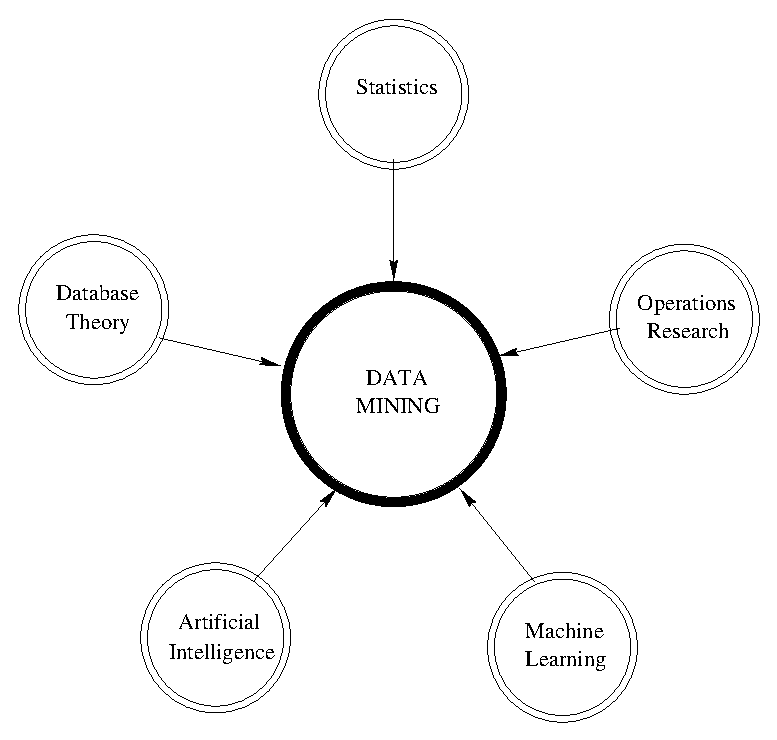
\includegraphics{../literature/dm_process.eps}}}
\caption{\label{fig:dm_process}Components of the Data
Mining Process}
\end{figure}
\index{Data Mining Components}  

\section{The Goal of the Thesis}\label{sec:int_hyp}
\index{Thesis Goal}

The ability to discover {\em knowledge} from a database which is not
explicitly represented in the data is clearly a desirable goal. We
propose that such {\em data mining} can be achieved using NDs,
generalisations of the FD, 
which themselves have a well-defined semantics for application within
the relational model. The application of NDs allow data
mining principles to be exercised on categorical data, often the bulk
of many corporate databases, or a combination of categorical and
numerical data. 

\smallskip
We show how relations containing indefinite or temporal data satisfy
numerous ND sets, being either definite instances of indefinite data
or possibly changing ND sets over time. The ND sets satisfied are
obtained from an initial template of FDs which is supplied by the
user; alternatively, it would be possible to mine for ND set
satisfaction. In the indefinite
domain the ND sets are satisfied in definite instances of the same indefinite
relation. We show how {\em resampling}, a computationally
intensive sampling procedure, may be applied on increasing sample
sizes to determine an approximate fixpoint upon which a heuristic based
hill-climbing algorithm is employed to find a suitable ND set
approximation to functional satisfaction. 
In the temporal domain the ND sets may change over time
for the same attributes; we
show how resampling and other time series statistics may be employed
to determine {\em properties} which may hold over time, using a logic
we have developed. Our data
mining framework thereby discovers information using many ND set
approximations upon which statistics are applied, varied for the
domain in question, to make further inferences from the data.

\section{Knowledge Discovery in Databases and this thesis}\label{sec:int_kdd}
			\index{Knowledge Discovery!Goals}
			\index{Knowledge Discovery!Outline}
			\index{Machine Learning!and Data Mining}
			\index{Pattern Discovery}
			\index{Data Warehouse}

 
\begin{figure}
\centerline{\scalebox{0.5}{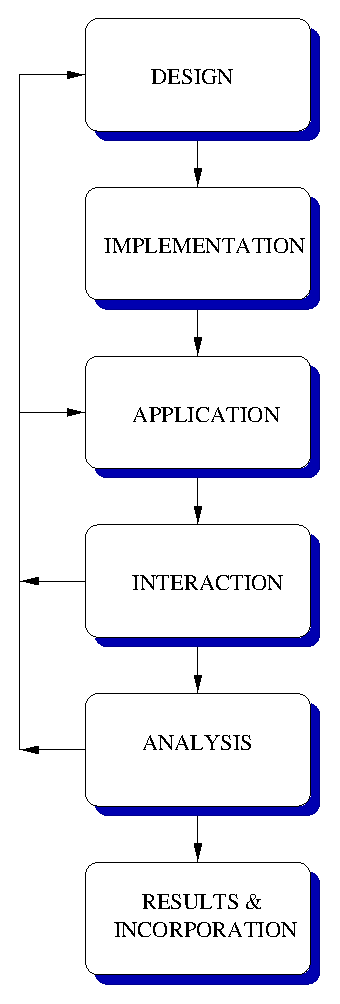
\includegraphics{../literature/kd_process.eps}}}
\caption{\label{fig:kd_process}The Knowledge Discovery
Application Cycle}
\end{figure}

The following widely accepted definition is due to \cite{kdd96}:

\begin{definition}[Knowledge Discovery in Databases]
\begin{rm} Knowledge Discovery in Databases is defined as {\em the
nontrivial extraction of valid, previously unknown, potentially
useful, and ultimately understandable information from a database}.    
\end{rm}
\end{definition}
\index{Knowledge Discovery!Outline}		

Knowledge Discovery may only provide {\em potentially} useful
information given that it may frequently discover relations, possibly
weak, between unconnected real-world information or even relations
that do not serve the interests of the user.  This includes the
possible discovery of redundant information. For instance, in a
medical database a system may discover a dependency $pregnant
\rightarrow female$ implying that all pregnant patients are female;
obviously such information is superfluous. Methods 
to prevent such redundant information generation may include the
specification of trivial associations before the mining process takes
place and continuous interaction with an expert, a much understated
component of knowledge discovery, defined as {\em data
archaeology} \cite{ba96}, as well as provision of a dependency
template upon which knowledge is discovered.   

\medskip
Knowledge discovery comprises a number of component parts including
data cleansing, design, warehousing and mining as well as expert
analysis, detailed in Figure~\ref{fig:kd_process}. Databases within
data warehouses are now frequently designed with a view to data mining
operations; where the goal of the database is {\em reliable storage}
the goal of the data warehouse is {\em decision support}
\cite{fay98b}. The process of data cleansing includes collecting data 
from different sources and processing it into a homogeneous form. The
design and implementation of a capable knowledge discovery tool will handle
these stages. Figure~\ref{fig:kd_process} displays a generic cycle
for knowledge discovery. It highlights the requirement that
interaction and analysis of the system may need to return to the
design stage if initial results suggest comparison with new data, which
may have been omitted, or the data cleansing stage has to be repeated
with new error parameters, perhaps to adjust the error and confidence
for noise within the database.  
Recent work has included
research on formalising the data warehouse \cite{hgmw95,inm96a} as
well as significant
data cleansing research.  Interesting as the issues of data
cleansing and warehousing are, we do not consider them further within
this thesis, concentrating on data mining.

\medskip

Knowledge
discovery refers to the process of extracting patterns and relationships 
from the data whereas data mining refers to the actual process of applying
these algorithms to the data, though many of the boundaries are vague.
In data mining applications a key requirement is 
the preparation of data for analysis. In Figure~\ref{fig:kd_process},
an example of a KDD application cycle, we assume that the
design and application components handle any required data
cleaning. Many data mining algorithms may also divide the data into
suitable training and validation subsets.   
Data Mining encompasses a number of different
approaches, such as clustering, data summarisation, learning
classification rules, finding dependency networks, 
and anomaly detection.  Data Mining is seen as a research frontier
for both database research and machine learning. Many other AI based techniques, such as Natural Language 
Processing and Distributed AI methods, are also increasingly included
\cite{kdd96}.  Machine Learning can be said to be the use of {\em
sophisticated} algorithms to generate and then process information,
for eventual understanding. \cite{xiao95} characterises learning from a
database as a triple $\langle$ D, C, A $\rangle$ where 
D is the data, C the {\em concept biases}, and A the language in which to
phrase the definitions. He also notes that as a database stores no  
negative information induction should be performed cautiously to avoid
over generalisation.
\medskip

Data Mining has been defined as the application of algorithms, within
the limits of computational efficiency, that produce a set of
expressions $E$ which represent patterns expressed in a well-defined
language over a data set $F$ \cite{kdd96}. There are a number of ways to
represent $E$, including: association rules \cite{ais93,toi96b}, rough
sets \cite{ziar91,incunc93}, temporal logic \cite{pt96,bt98}, and
FDs \cite{km95}. This 
latter class consists itself of many well-developed approximation
techniques including Fuzzy FDs \cite{bdp94}, PAC-approximation
\cite{at94,km95}, and probabilistic approximations
\cite{psm93,pk95,hkp98}. To this category we add NDs for pattern
expression \cite{cl98}. Their suitability to this task is shown via
their satisfaction of {\em lattice properties} from which measures for
approximation can be formed and the desirability of
mining NDs from databases. Mined NDs, expressed as {\em cardinality
constraints} (equivalent to NDs with empty left hand sides), have
recently been used to
reverse-engineer ER-models in \cite{sou98}. We also develop a
restricted temporal logic for discovery of patterns using NDs as our
atoms \cite{cl98f}.

\medskip

To date knowledge discovery research has focused on application
within relational databases containing definite information. However,
the advanced functionality of DBMSs extend the set of
data types beyond that of strict numerical or categorical data to
include NULL value representation \cite{lip79,il84}, the most common
interpretation being that a value
exists but we do not currently know what it is. The literature has
extended this to handle indefinite or disjunctive information where a
value might now be, for example, Tuesday or Wednesday, implying that
we know the value is one of a finite set \cite{inv91,vn95}.  To allow DBMSs to
handle scheduling 
and planning processing and querying directly the ability to store 
indefinite information is paramount. Data Mining techniques will then
have to be extended to encompass these data types. We show for the
case of NDs in \cite{cl98} how definite instances (or possible worlds)
of an indefinite relation satisfy different ND sets; other
FD approximation methodologies can be applied similarly.

\medskip
\index{Data Mining!Introduction}

Data Mining algorithms are bounded both by potentially huge data sets
and the limits of a computationally efficient methodology. Therefore,
sampling and the use of randomised algorithms for data mining have
been utilised \cite{km94,gms97,cl98b}. Sampling within data mining has
been well studied \cite{km94,jl96}; to this we include the use of
resampling for data mining. Resampling is a computationally intensive
sampling methodology for non-parametric data; the distribution is
unknown for most data sets. Its use allows for information about the
distribution of data to 
be made and has a wider range of application than standard
sampling. Many data mining algorithms seek to make inferences from
sample data; classical statistics refers to this as {\em estimation}. 
Our work incorporates resampling processes \cite{efro79,et86,et93}
to achieve this. Heuristics are often required for knowledge to be
discovered;
in such cases randomised algorithms may allow the efficient processing of
data for discovery. Indeed for a theory to be verified without error
the complete data set needs to be examined though only one violating occurrence
is required for falsification. Randomised algorithms and sampling allow for 
efficient analysis to be achieved utilising this fact. We use randomised
algorithms and resampling to find approximate solutions to the
{\em consistency problem}, known to be NP-complete, which is the problem of
searching for a possible world within an indefinite relation that
satisfies a given FD set \cite{vn95,cl98b,cl98}.

\medskip

Temporal
Databases have been a significant area of research in the last few
years \cite{tcg93,ct95}, unsurprising given the need for temporal
support in real-world applications, particularly in the financial and
medical domains. Building on this work is the rapid rise of, and need
for, temporal data mining applications.  
Much of Temporal Knowledge Discovery relates to forecasting events in the
future and analysing 
patterns which occur over time. Indeed, these goals are closely
related to time series analysis, a well established research field in
statistics and econometrics \cite{end95,naze88}. Nearly all databases
in use contain a 
temporal component and there has been much recent data  mining work on
temporal knowledge discovery \cite{alss95,pt96,bc96,bt98}. 

\medskip

Data mining and statistics have been substantially analysed
\cite{fhs96,gmp97}. One of the prime goals of data mining
is that of predicting values and this is inherently related to the
representation of temporal data and {\em time series analysis}. Time
series analysis when applied in a 
 database is used for anything from identifying demand and modifying
supply accordingly or for calculating patterns and changes in salary over time
to predicting the expense of projects within different time
periods. Until recently there was minimal use of time series analysis
techniques within temporal databases \cite{smd95}.

The Classic multiplicative model views time series as containing four
parts, namely trend, cycles, seasonal, and irregular patterns.
Trends may be up or down and can be used to characterise the time
series over a long time irrespective of short term fluctuations.
Cycles display a recurring up and down movement around trend levels,
including expansion and contraction. Seasonal patterns complete within
a given time period. Finally, irregular patterns account for erratic
changes in a time series and may be modelled as noise in the data.
\smallskip

The above may be understood using many techniques including trend
moving averages, ratio-to-moving averages (for deriving 
the seasonal component), and difference equations for model
representation. Using these time series may be extrapolated.
Related issues are (1) granularity changes (2) application of moving
windows, and (3) attribute value transformation. The temporal logic we
present, as well as the related work we survey
\cite{frm94,lai93,alss95,dgm97,dlm98}, is closely linked with many
aspects of (stationary) time series analysis. \cite{gmp97} also
tackles the issues of how data mining is extending and not simply
repeating previous statistical research. There have been significant
use of data mining algorithms incorporating statistical
functions, not least in the scientific domain on applications as
diverse as astronomical cataloguing through to geological sensing for
earthquake detection \cite{fhs96}.

\medskip

Recently there have been a number of different approaches to temporal
data mining, stemming from machine learning work on pattern
matching \cite{lai93,alss95}. There seems to be a demarcation between research based on
data mining from temporal databases and research using time series as
the input data set from which knowledge is to be discovered. Our
approach allows for discovery from either or a combination of the
two, given that in each case only series of
numbers change over time. 

\medskip

Temporal logic is used for temporal data mining in
\cite{pt96,bt98}. It has been shown to be sufficient for expressing
temporal relationships that have been discovered. If more complex
relationships are required, such as, say, correlation between two data
sets temporal logic does not have the functionality to express this
without an explicit {\em correlation function}. Therefore
we present a logic with statistical
functionality so that such values are embedded within the logic. Given
that the sentences of the logic express results of statistics
we do not have to present {\em confidence} and
{\em frequency} values (akin to work
on association rules \cite{ais93,kmrtv94,hkmt95}) for the rules that
we discover as our rule discovery 
itself is representative of specific statistical values. Our work on
temporal relations is pattern focused; we do 
not attempt to discover a global model, the undoing of many time
series analysis studies, but logical rules which describe local behaviour
on subsequences of the temporal data set. Of course these can be, if
desired, extended to global conditions.
It is interesting to note that discovery in this
sense is closely linked to the power of the query language. Similarly,
we may view rule discovery using temporal logic directly dependent on
the expressiveness of the logic.
Patterns within a (temporal) database may be referred to as {\em properties}
which model the data. Temporal logic for property satisfaction is a
well-researched area within program verification. Properties used to
express the correctness of a temporal system also have application
in data mining where a database with many states may be viewed as a
temporal system. We claim that these properties are therefore suitable
as {\em candidate patterns} for potentially interesting knowledge
discovery. 

\medskip

The real-world desire for ever more information and knowledge
precludes data mining from being anything but a significant research
area. Many different mechanisms for expressing patterns have been
developed and we believe that NDs, though not a panacea for expression
within data mining, are widely applicable and easily understood. 
To illustrate, an ND $STUDENT \to^5 COURSE$ in a timetable relation
specifies that a student can take at most 5 different courses; it is
clear that such data may often need to be represented and in current
DBMSs this data would satisfy no constraints.
The progression towards a standardised query language for data mining
\cite{cha98} 
would benefit from their inclusion as we note their utility in
different domains.

\section{Main Results and Contribution}\label{sec:int_contrib}
\index{Thesis Contribution}

We provide a novel approach to data mining. We show how, in databases
containing indefinite and temporal information, given an FD set F we
form sets of approximations to F which may be satisfied for
different definite instances of the indefinite relation or over time
in a temporal relation. We choose to express these approximations as
sets of NDs;
other expressions may also be appropriate, such as a probabilistic
approximation \cite{psm93}. In either indefinite or temporal databases
we can use these sets to obtain statistics to determine how they
may change in the indefinite relation or over time. We show
how resampling can be applied to these sets to make inferences from
the data. For indefinite relations we present a dynamic resampling
process which allows for resampling on increasingly large sample sizes
until an approximate fixpoint is reached. This provides an upper bound
on sample size which is then used in a heuristic based hill-climbing
algorithm. 
For temporal relation
sequences we may take moving averages or create resampled sequences to
determine how patterns, expressed in the form of {\em properties}, are
satisfied at various time points. 

\medskip

We now outline our methodology as a general framework. We
take a large set $\alpha$ of approximations to a given FD set and then
apply resampling to 
$\alpha$ to draw conclusions on the nature of the data in the
database. The exact method of the application of resampling, and the
use of other statistical functions, differs with the type of data we
are mining. This framework is applicable to other domains, extending
the traditional mining approaches of simply using approximations to
dependencies to infer information. Indeed, we assume that an FD set is
provided by the user as a template in both indefinite and temporal
domains; this FD set may be modified by a system user to compare
results for different dependency sets. We shall demonstrate how it is
possible to utilise temporal and indefinite domains from which the
approximations, in our 
case NDs, are taken to make further discoveries from the relation
which is being mined. 

\smallskip
\noindent This thesis makes the following specific contributions:
\begin{enumerate}
\item NDs are shown to be effective and useful for 
data mining in that they provide a clear notion of proximity to FDs.
NDs are shown to be able to efficiently and accurately approximate FDs
in a relation with an easily understood semantics. 
An evolutionary database design procedure is introduced as a 
motivation for real-world ND applications as a precursor to their application
in non-standard database domains. The lattice properties of NDs are
exploited to provide a metric for data mining which we use in this work. 
\item We provide a detailed study on an approach which uses NDs to
provide approximations to the Consistency Problem, namely the
NP-Complete problem of finding a definite world that satisfies a set
of FDs within a relation containing indefinite data. 
\item Procedures for applying the Bootstrap within relations containing
indefinite and temporal data are defined and shown to be useful via extensive
simulations. They include a dynamic procedure for application of the
bootstrap in indefinite relations for sample size determination. 
\item A temporal logic for NDs is presented. This logic is then used
for mining sequences of relations. We examine the sequences for proximity
to FD set satisfaction, expressed as NDs, and compare this
to standard time series 
analysis. The logic is transferable to standard time series and other
linearly ordered numerical data sequences.
\item We present a model for the application of our temporal data
mining system to a sequence of temporal relations. Results using
financial time series of stock prices from the oil,
finance and retail sectors are presented and analysed.
\end{enumerate}

The thesis also presents a taxonomy of standard and temporal 
dependency data mining, placing our work in context, as well as making
suggestions for future research. 

\section{Outline of the Thesis}\label{sec:int_outline}
\index{Thesis Outline}

After this introduction, Chapter~\ref{chap:review} formally presents
the required relational database theory so that the remainder of the
work is self-contained.  All of the relevant theory presented is
placed in the context of this research and related work. Additionally,
we present related data mining research, focusing on three areas:
\begin{enumerate}
\item
We examine functional dependency data mining and the methods used to
find approximations to FDs \cite{km95,at94,Mann92,sf93,HS95,pk95,bel95b,psm93}, of which using NDs is part of our
contribution, shown in Chapter~\ref{chap:numdep}.
\item We briefly
examine work conducted on 
indefinite information, related to our study of the consistency
problem.
\item Temporal data mining research is discussed so that
the reader is able to appreciate the contribution of the
work in Chapters~\ref{chap:templog}
and~\ref{chap:tempresult}. 
\end{enumerate}
Chapter~\ref{chap:review} concludes with a
brief presentation of
resampling in statistical applications, which is then expanded upon in
Chapters~\ref{chap:consistency} and~\ref{chap:tempresult}.

\medskip

Chapter~\ref{chap:numdep} presents ND theory with regard to data
mining, including a {\em chase procedure} for NDs. The chase
procedure may be used to modify a relation to satisfy a given ND set
allowing us 
to test whether or not an ND set implies a specific ND.
We show how a
data mining distance function is used for assessment, related
to approximation work presented in
Chapter~\ref{chap:review}. Additionally, research on applying NDs for
mining within relations is discussed and compared with other
approaches. We also present a practical database design tool for randomly
evolving example relations which satisfy FD sets.

\medskip
Chapter~\ref{chap:consistency} then introduces
the consistency problem and its applications. We present randomised
algorithms which use NDs and the chase procedure for indefinite
relations together with a novel application of resampling to determine
sample size. We present results of extensive simulations applied to
randomly generated indefinite relations. We also discuss the
usefulness of the chase procedure as a heuristic.

\medskip

Chapter~\ref{chap:templog} moves on to temporal data mining. We
motivate the need for rules in temporal data mining, introduce our
logic for temporal data mining, examine the logic and introduce the
notion of temporal properties which we use in our temporal data mining
environment. This logic is then assessed against a standard time series
analysis which could be conducted on any time series data set and also
on any temporal sequence of relations satisfying ND sets in each
state over fixed intervals. Chapter~\ref{chap:tempresult} presents the
details of our temporal 
rule discovery system, the use of resampling, and results from data
sets studied, concluding with a discussion of future work together
with an analysis of the utility of our temporal data mining approach.

\medskip

Finally in Chapter~\ref{chap:conclusion} we give our concluding
remarks and present a final discussion of the work, introducing
avenues for further research and stating the open problems that remain.


\section{Notation}
\index{Notation}

We present an index of the symbols used at the beginning of the thesis
in the symbol index.

\smallskip

This thesis adheres to the standard notational convention generally followed in
relational and deductive database texts.  R refers to a relation
schema, denoting a finite set of attributes,  and $r$ to a relation over R,
denoting a finite set of tuples.  Uppercase letters (possibly
subscripted) refer to attributes if they are from the beginning of the
alphabet such as A, B, C and to attribute sets if they are from the
end of the alphabet such as X, Y, Z.  Tuples are referred to by
lowercase $t$ and $u$ (possibly subscripted).

\medskip

Lowercase letters (possibly subscripted) refer to constants if they
are from the beginning of the alphabet such as $a$, $b$, $c$ and to
variables if they are from the end of the alphabet such as
$x$,$y$,$z$.  Predicate symbols (possibly subscripted) of arity $\ge
0$ are referred to by $p$, $q$ and $r$. 
We use $\mid X \mid$ to refer to the cardinality of set $X$ and simply
$X$ to denote the singleton set $\{ X \}$. The nonempty powerset of a
set $X$ is denoted by $\cal P$($X$). From the 
relational database literature, we refer to the union of
two sets $X \cup Y$ by $XY$. 


